\input{../../../slides.sty}
\begin{document}
\begin{frame}
    \begin{figure}
        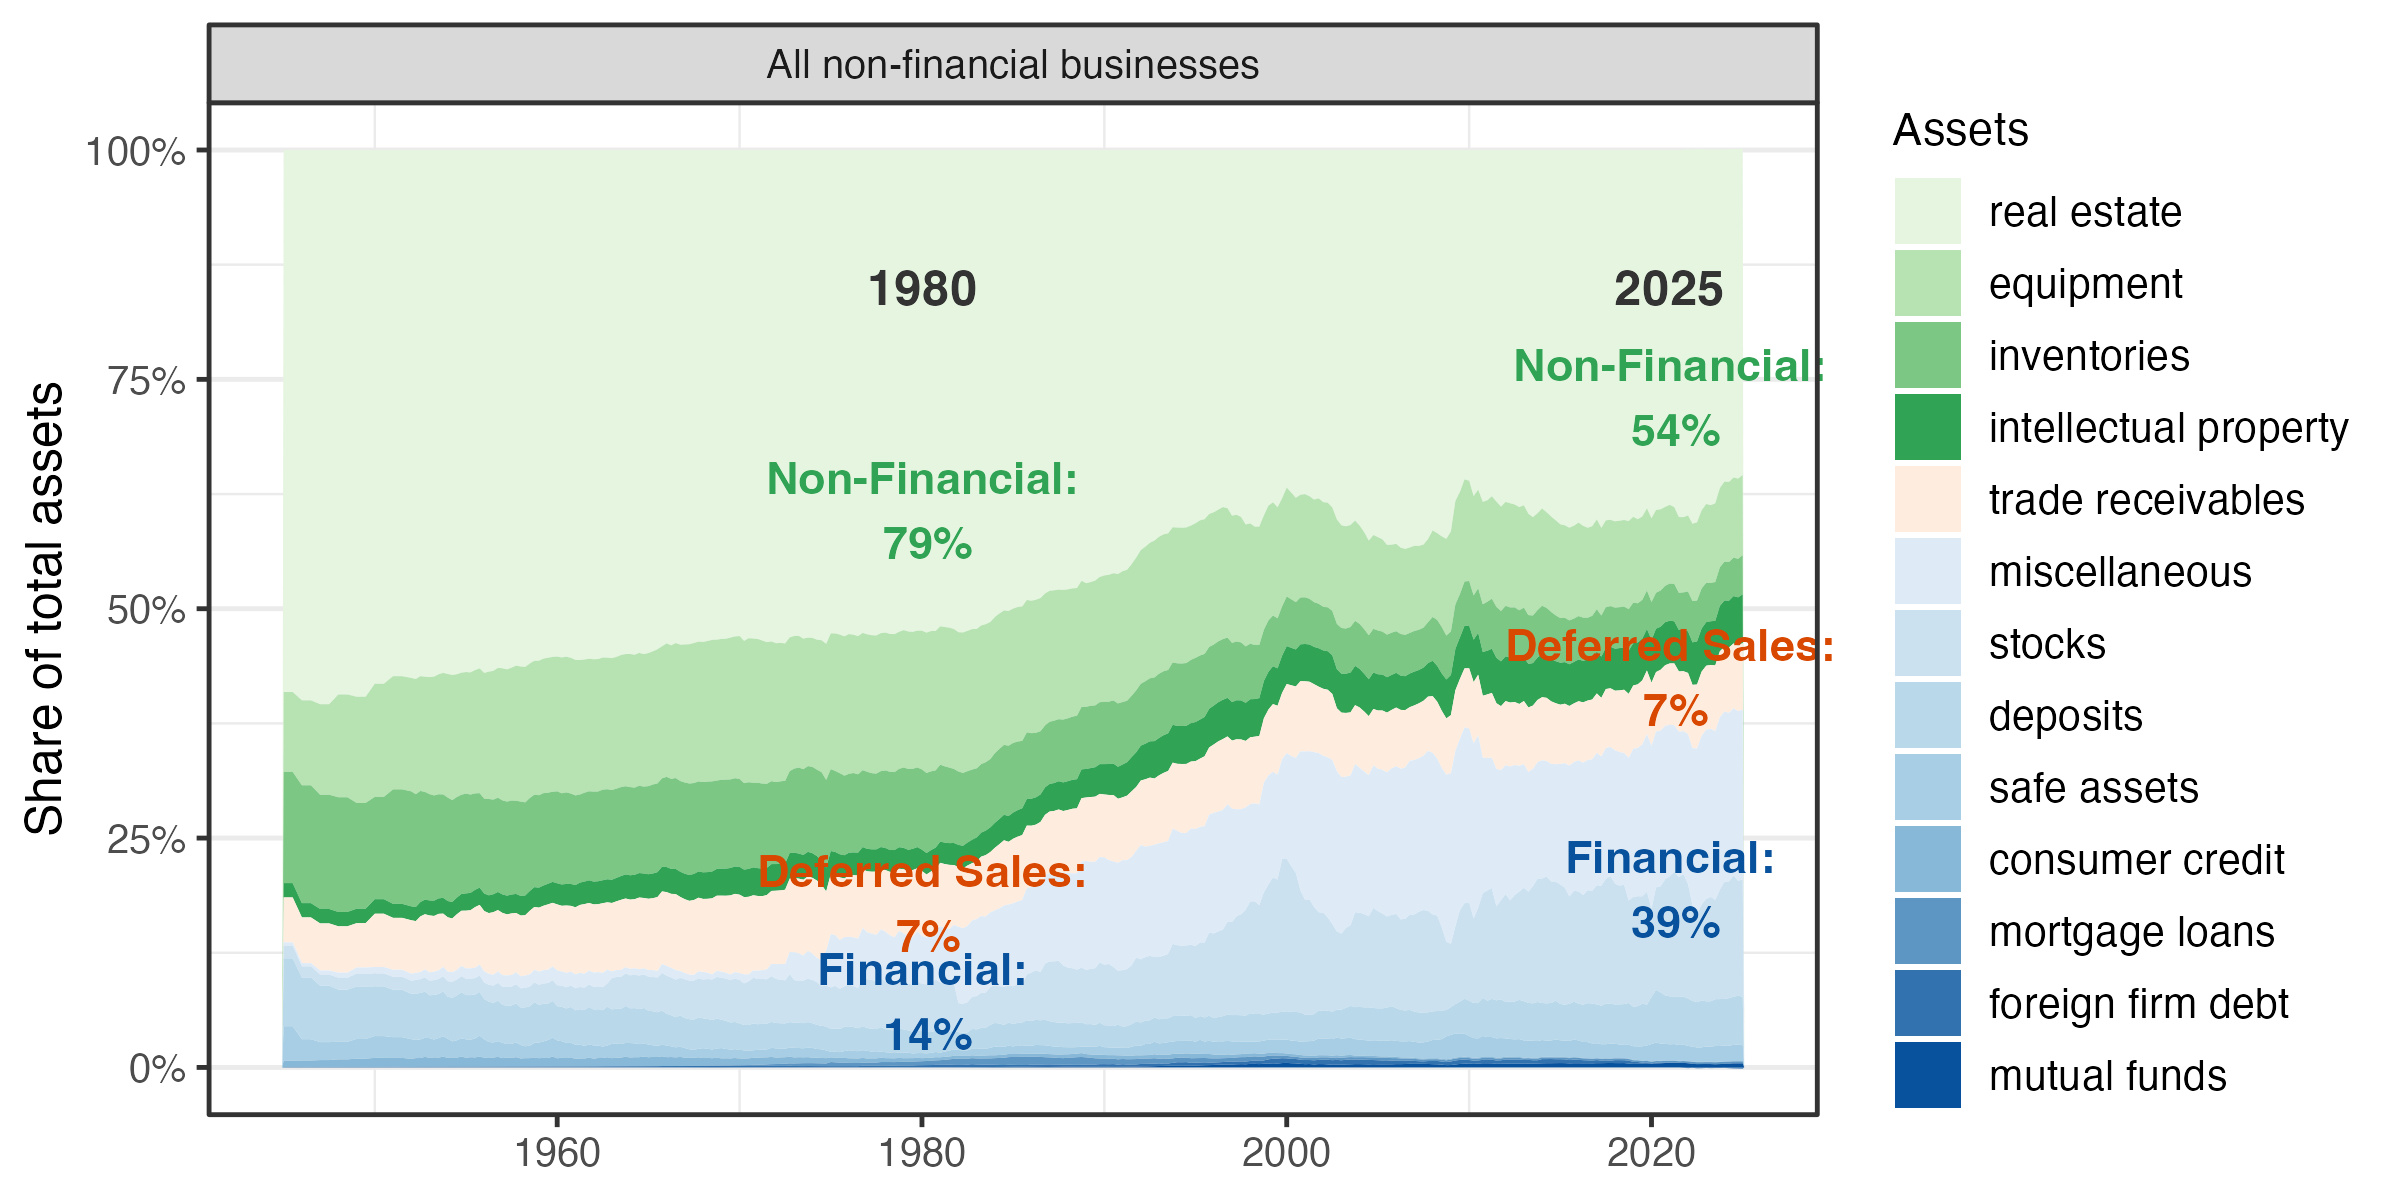
\includegraphics[height=.8\textheight]{../figures/exploration/firm-assets/assets_allbusiness.png}

        Non-financial firms' assets got more financial since 1980. 
        
        \footnotesize Mostly stocks and ``miscellaneous.''
    \end{figure}
\end{frame}
\begin{frame}
    \begin{figure}
        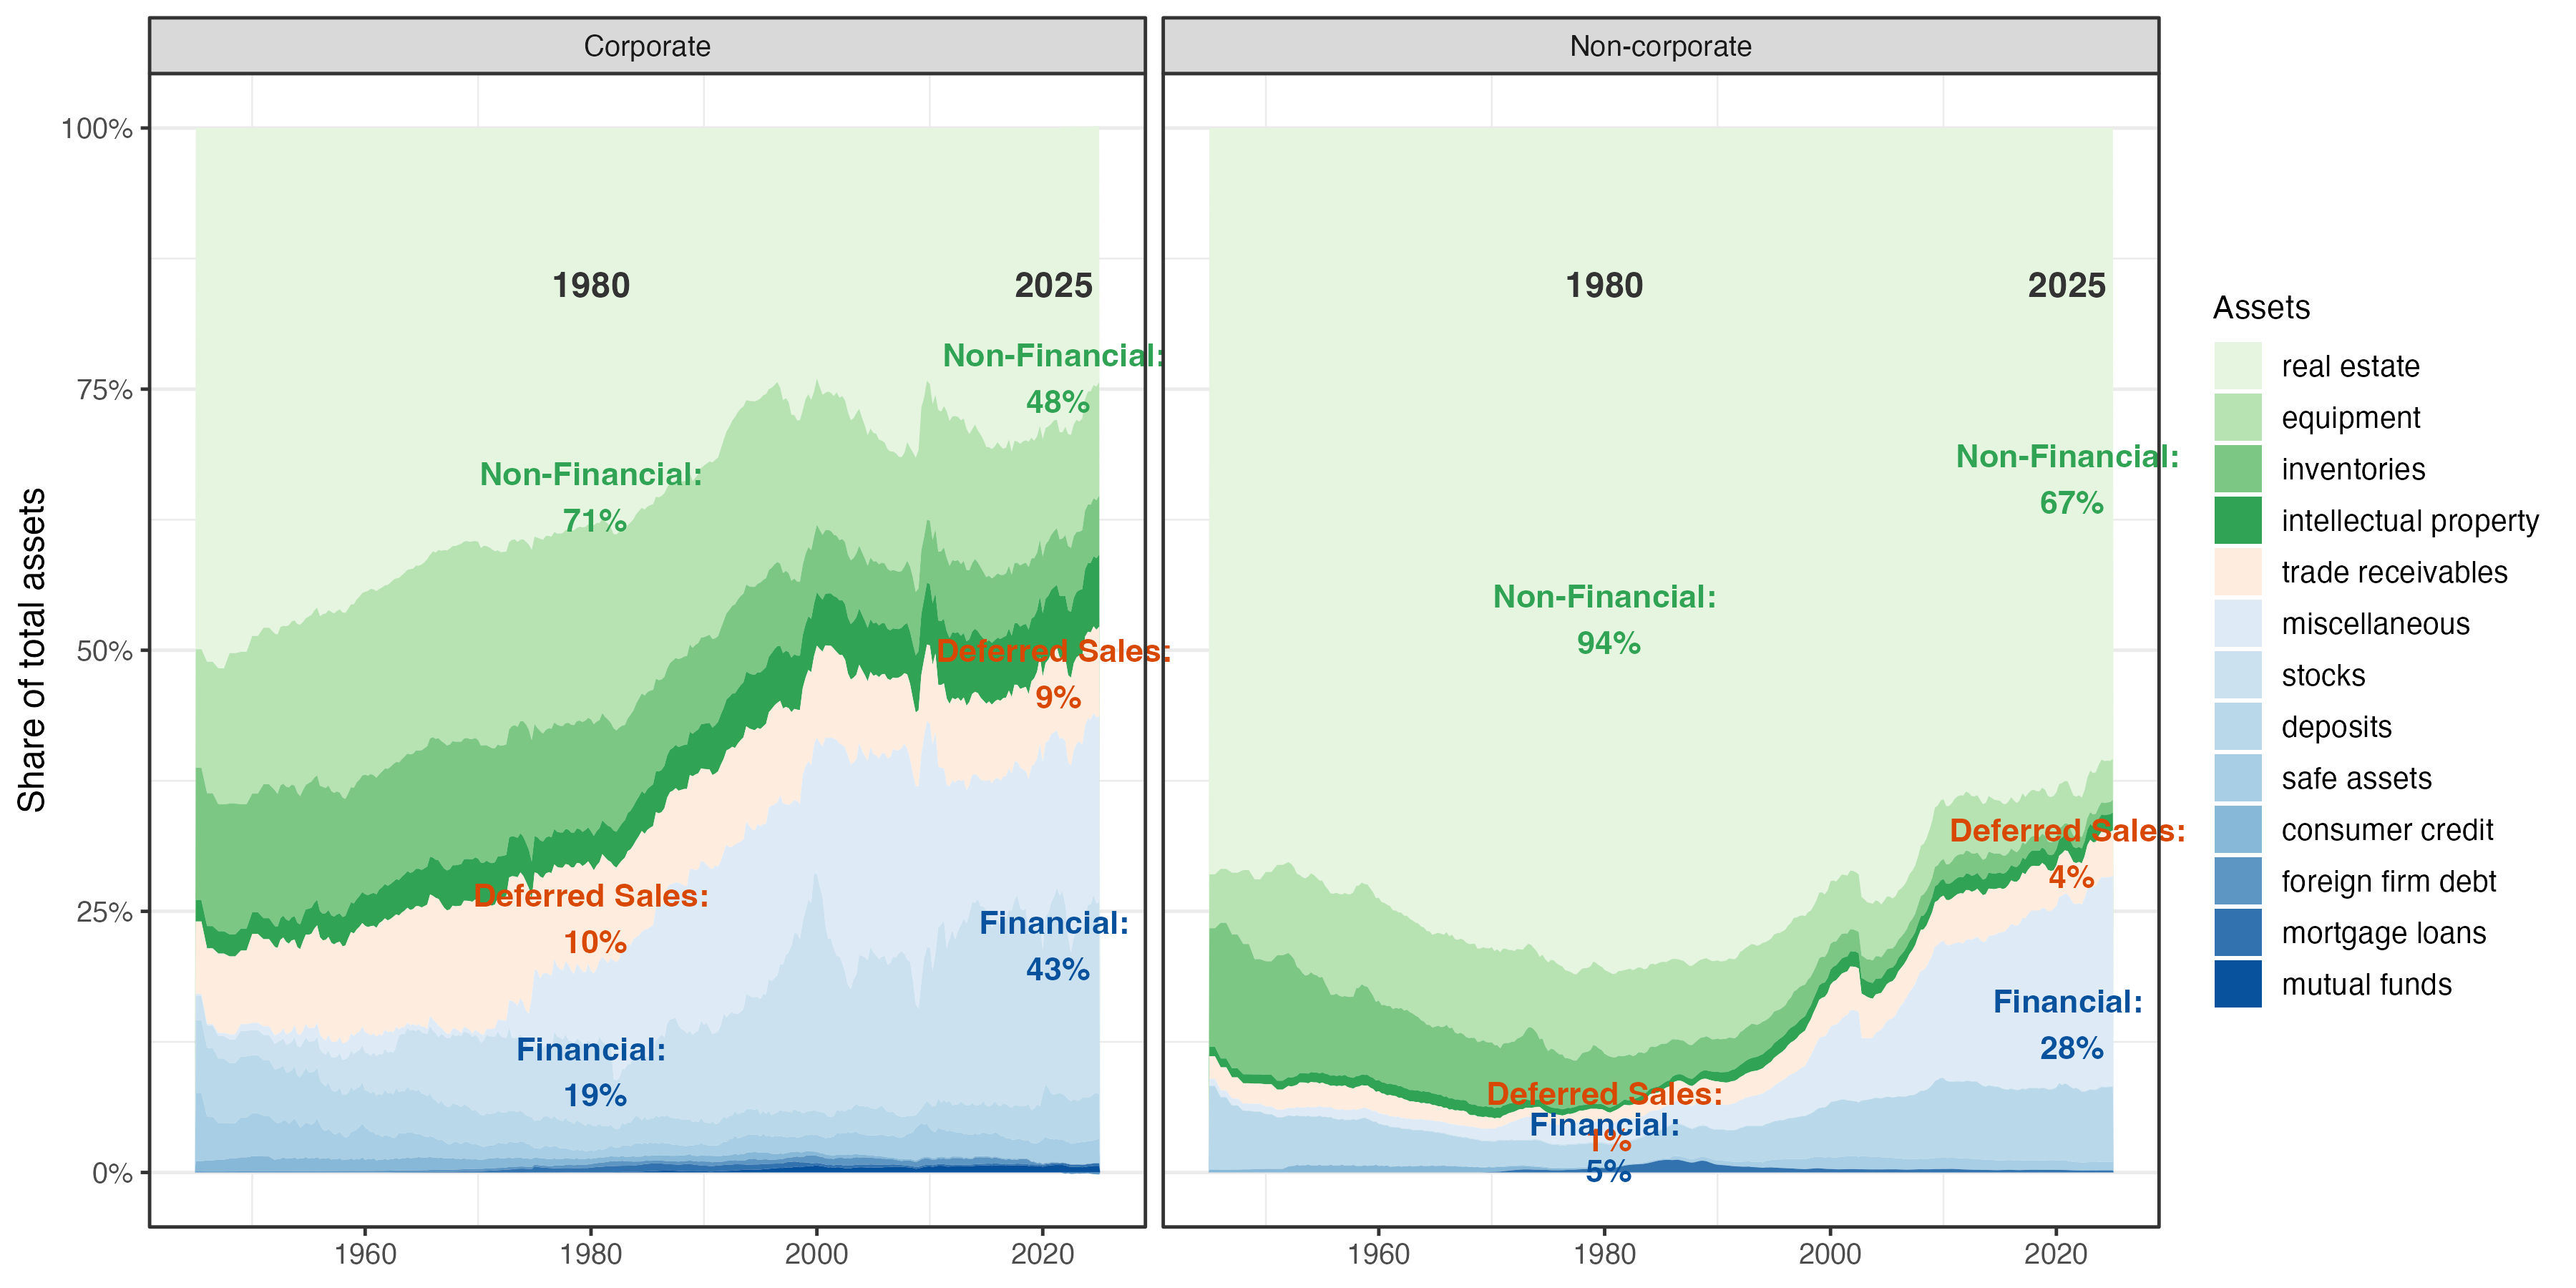
\includegraphics[height=.8\textheight]{../figures/exploration/firm-assets/assets_corporate_noncorporate.png}

        True for both corporates and non-corporates.
    \end{figure}
\end{frame}
\begin{frame}
    Is this because more financialized sectors became more dominant?
    
    Or because every sector became more financialized?
\end{frame}
\begin{frame}
    \begin{figure}
        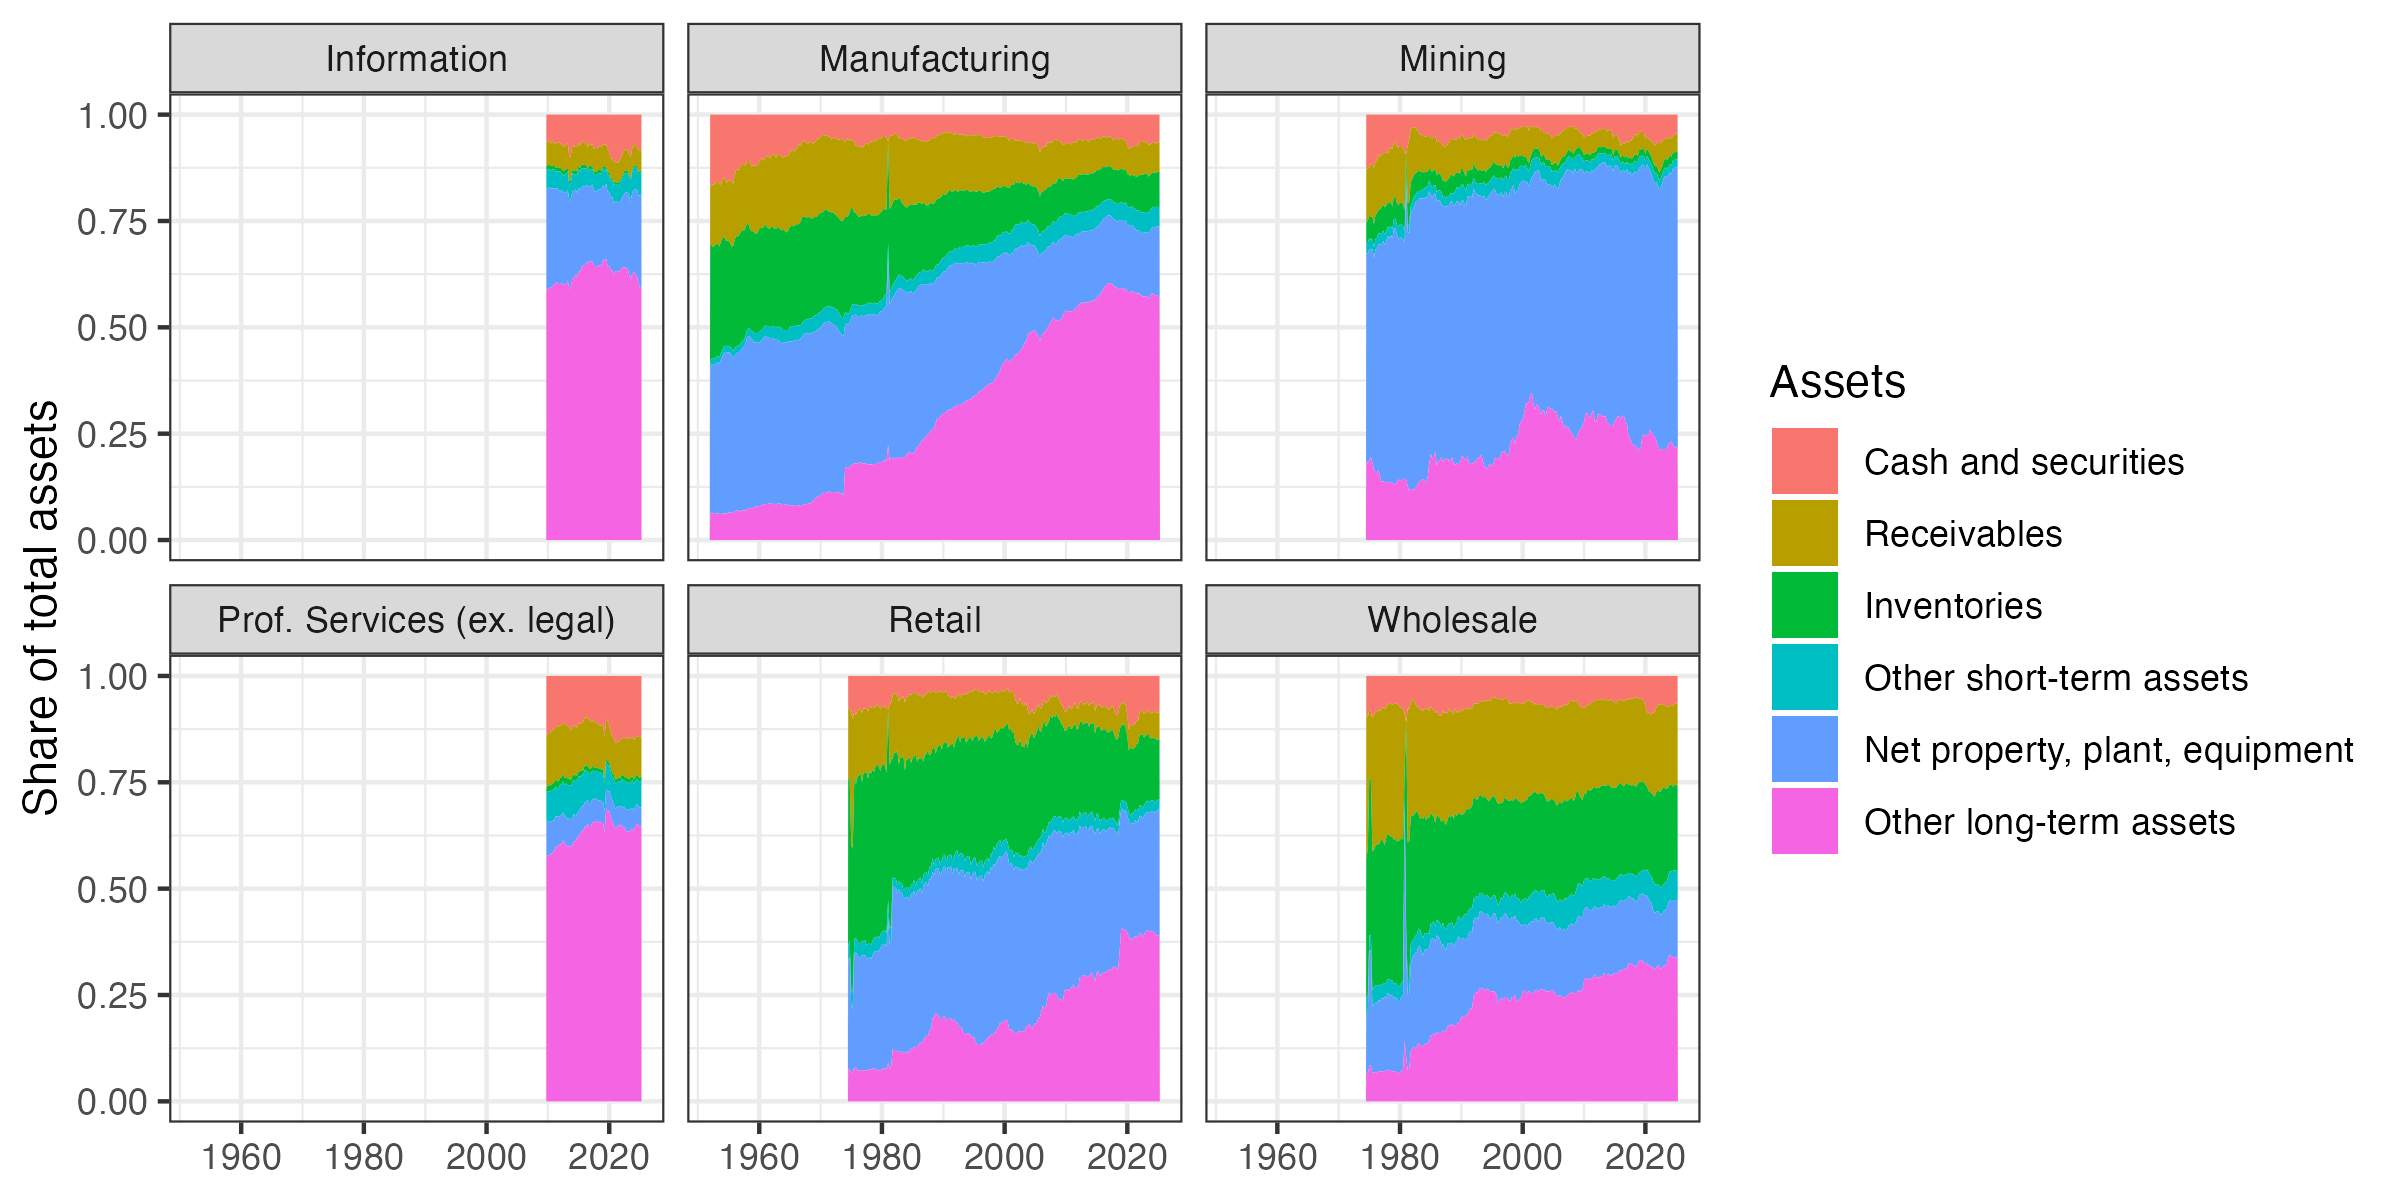
\includegraphics[height=.8\textheight]{../figures/exploration/firm-assets/QFR_bsheet_assets.png}

        Unclear - long-term (noncurrent) assets includes both non-financial intangibles and long-term financial investments.
    \end{figure}
\end{frame}
\end{document}